\documentclass[serif, 12pt]{beamer}

\usepackage{graphicx} % Allows including images
\usepackage{booktabs} % Allows the use of \toprule, \midrule and \bottomrule in tables
\usepackage[utf8]{inputenc}
\usepackage{amsmath}

\setbeamertemplate{navigation symbols}{}%remove navigation symbols
\setbeamertemplate{footline}[frame number]
\setbeamerfont{page number in head/foot}{size=\normalsize}



\title{Spectral Graph Drawing}
\author{Rodrigo Arias}
\date{\today}
%\date{}

\begin{document}

% FW = Final Work (graded from 0 to 10) in which each participant is required to
% present a research paper or section of a book (previously assigned by the
% lecturer).
%
% The presentation consists of:
%  * 3-5 minutes background on the topic of the paper, a motivation.
%  * 1 minute overview of the key ideas of the paper.
%  * 15 minutes presentation with most important details.
%  * 5 minutes demo of a program that implements the ideas introduced in the
%    paper. 

\begin{frame}
	\maketitle
\end{frame}

%\begin{frame}[plain]
%	\makebox[\textwidth]{\includegraphics[width=\paperwidth]{pugh-fire}}
%\end{frame}

\begin{frame}{Outline}

\begin{itemize}
\item Background
\item Motivation
\item Ideas from the paper
\item Methods
\item Examples
\item Conclusions
\end{itemize}

\end{frame}

\begin{frame}{Background}

The placement problem.

\begin{center}
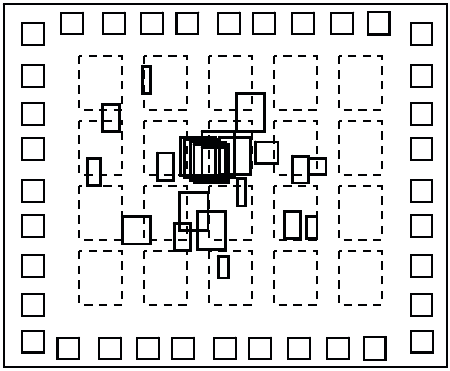
\includegraphics[scale=0.3]{analytic-placement.png}
\end{center}

\begin{itemize}
\item Analytic solution: Minimize an \textbf{objective function} (wire, area...) 
via mathematical analysis.
\item Global placement must be legalized afterwards (detailed placement).
\end{itemize}

\end{frame}

\begin{frame}{Motivation}

\begin{center}
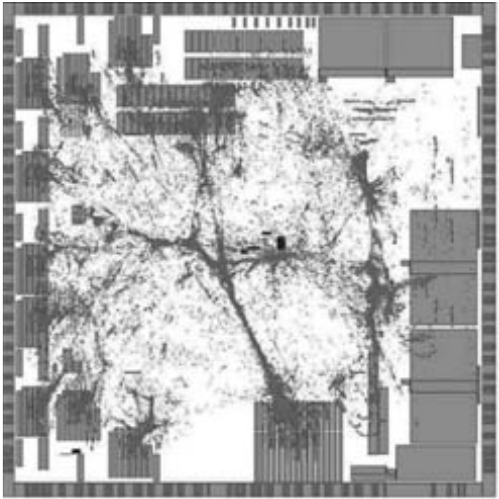
\includegraphics[scale=0.3]{lots-cells.png}
\end{center}

\begin{itemize}
\item Cells and nets can be modeled as an undirected graph
\item Spectral methods can be used to draw complex graphs
\end{itemize}

\end{frame}

\begin{frame}{Ideas from the paper}

In the Koren paper \cite{koren} two methods to find the placement of the nodes 
are described, using the following properties.

\begin{itemize}
\item Method 1: The Laplacian matrix $L$
\item Method 2: The normalized Laplacian matrix $\mathcal L$
\end{itemize}

The methods minimize the total \textbf{wire-length}

\end{frame}

\begin{frame}{Method 1: Laplacian matrix $L$}

\begin{itemize}
\item A graph can be represented by the adjacency matrix $A$, were
$$ a_{ij} =
\begin{cases}
	1 & \text{if $i$ and $j$ are connected} \\
	0 & \text{otherwise}
\end{cases}
$$
\item Also, the degree matrix $D$ has the degree of each node in the diagonal, 
$d_{ii} = deg(i)$.

\item Finally the Laplacian matrix is defined as $L = D - A$
\end{itemize}

\end{frame}

\begin{frame}{Method 1: Laplacian matrix $L$}


\begin{itemize}

\item The problem is formulated as the minimization of the square wire-length
\begin{equation}
\begin{split}
\min_x \  & E(x) = \sum (x(i) - x(j))^2 \\
\textrm{s.t.} \ & \textrm{Var}(x) = 1
\end{split}
\end{equation}
\item The eigenvalues $\lambda_1 \le \lambda_2 \cdots \lambda_m$ and 
eigenvectors $v_1, v_2, \cdots v_m$ of $L$ are computed.

\item The positions of the nodes are given by the coordinates of $x = v_2$ and 
$y = v_3$.
\end{itemize}

\end{frame}

\begin{frame}{Method 2: Normalized Laplacian matrix}

\begin{itemize}
\item Let $d_i$ be the degree of the node $i$, we define the normalized 
Laplacian matrix $\mathcal{L}$ as:
$$ \mathcal{L}(i,j) =
\begin{cases}
	1 & \text{if $i = j$, and $d_i \neq 0$} \\
	-\frac{1}{\sqrt{d_i d_j}} & \text{if $i$ and $j$ are connected} \\
	0 & \text{otherwise}
\end{cases}
$$

\item We give more weight to the nodes with higher degree, in order to cluster 
neighbours around centric nodes.
\end{itemize}

\end{frame}

\begin{frame}{Method 2: Normalized Laplacian matrix}

\begin{itemize}
\item The solution is computed as before, but now using the matrix 
$\mathcal{L}$.

\item The eigenvalues $\lambda_1 \le \lambda_2 \cdots \lambda_m$ and 
eigenvectors $v_1, v_2, \cdots v_m$ of $\mathcal L$ are computed.

\item The positions of the nodes are given by the coordinates of $x = v_2$ and 
$y = v_3$.
\end{itemize}


\end{frame}

\begin{frame}{Examples}

In order to test the methods, some graphs were generated

\begin{itemize}
\item Small graph crafted by hand with 7 nodes.
\item Erdös-Rényi graph with 100 nodes
\item A FPGA network from a real Verilog TX module with 345 nodes
\end{itemize}

\end{frame}

\begin{frame}{Small graph}
\begin{center}
\includegraphics[scale=0.5]{G3-laplacian.pdf}
\end{center}
Using the method 1, the Laplacian matrix $L$.

Wire-length: 8.82
\end{frame}

\begin{frame}{Small graph}
\begin{center}
\includegraphics[scale=0.5]{G3-norm.pdf}
\end{center}
Using the method 2, the normalized Laplacian matrix $\mathcal L$.

Wire-length: 12.87
\end{frame}

\begin{frame}{Small graph}
\begin{center}
\includegraphics[scale=0.5]{G3-spring.pdf}
\end{center}
Using the directed force method (for comparison).

Wire-length: 9.40
\end{frame}

\begin{frame}{ER graph}
\begin{center}
\includegraphics[scale=0.5]{ER-laplacian.pdf}
\end{center}
Using the method 1, the Laplacian matrix $L$.

Wire-length: 417.97
\end{frame}

\begin{frame}{ER graph}
\begin{center}
\includegraphics[scale=0.5]{ER-norm.pdf}
\end{center}
Using the method 2, the normalized Laplacian matrix $\mathcal L$.

Wire-length: 722.86
\end{frame}

\begin{frame}{ER graph}
\begin{center}
\includegraphics[scale=0.5]{ER-spring.pdf}
\end{center}
Using the spring method (for comparison).

Wire-length: 599.69
\end{frame}

\begin{frame}{TX graph}
Generated using Yosys \cite{wolf} from the Verilog file \texttt{uart\_trx.v}.
\begin{center}
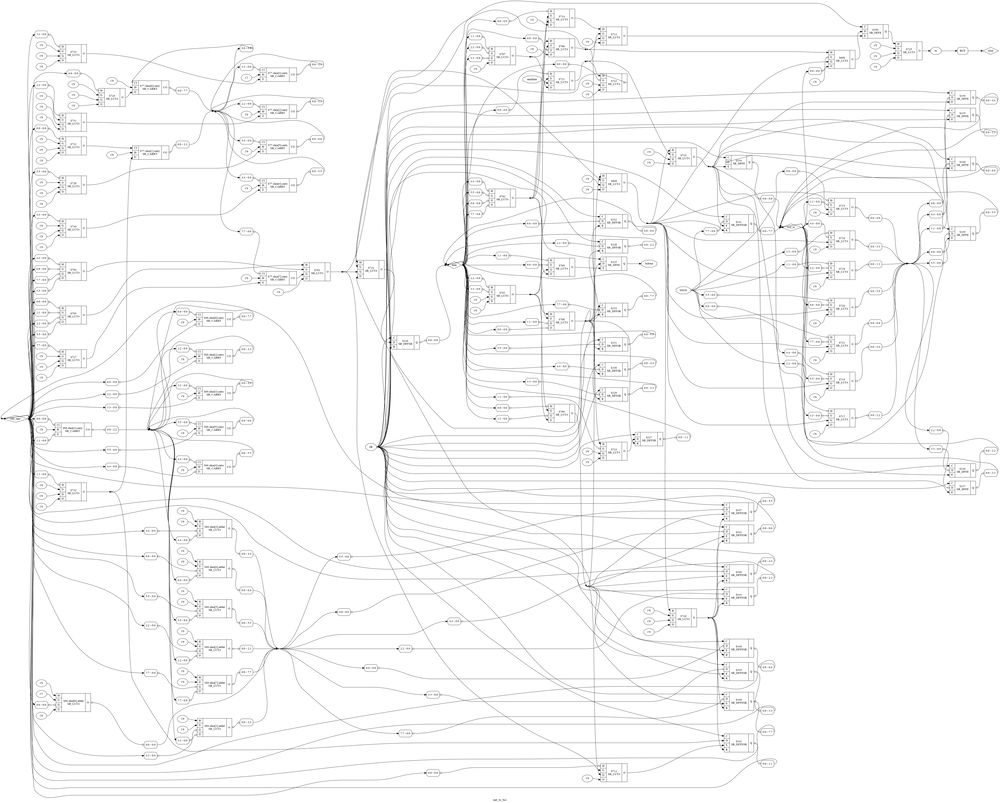
\includegraphics[width=0.7\textwidth]{uart-small.png}
\end{center}
\end{frame}

\begin{frame}{TX graph}
\begin{center}
\includegraphics[scale=0.5]{TX-laplacian.pdf}
\end{center}
Using the method 1, the Laplacian matrix $L$.

Wire-length: 78.78
\end{frame}

\begin{frame}{TX graph}
\begin{center}
\includegraphics[scale=0.5]{TX-norm.pdf}
\end{center}
Using the method 2, the normalized Laplacian matrix $\mathcal L$.

Wire-length: 733.78
\end{frame}

\begin{frame}{TX graph}
\begin{center}
\includegraphics[scale=0.5]{TX-spring.pdf}
\end{center}
Using the spring method (for comparison).

Wire-length: 172.13
\end{frame}

\begin{frame}{Observations}

\begin{itemize}

\item The proposed model doesn't take into account the size of the cells
\item Multiple cells can overlap in the same point
\item The behavior is not close to reality

\end{itemize}
\end{frame}

\begin{frame}{Conclusions}

\begin{itemize}

\item The spectral methods can be used in the global placement.
\item Don't produce great results in comparison with spring layout.
\item The underlying working principle is complex to understand.
\item May be suitable for larger graphs, as the matrices are usually very 
sparse.

\end{itemize}

\end{frame}

\begin{frame}{References}


\begin{thebibliography}{9}

\bibitem{koren}
Yehuda Koren
\textsl{On Spectral Graph Drawing}
Proceedings of the 9th Annual International Conference on Computing and 
Combinatorics, p496--508, 2003.

\bibitem{wolf}
Clifford Wolf, Johann Glaser.
\textsl{Yosys - A Free Verilog Synthesis Suite.}
In Proceedings of Austrochip 2013

\end{thebibliography}

\end{frame}

\end{document}
